\subsubsection{UC2 - Aiuto comandi}
	\begin{figure}[h]
		\centering
		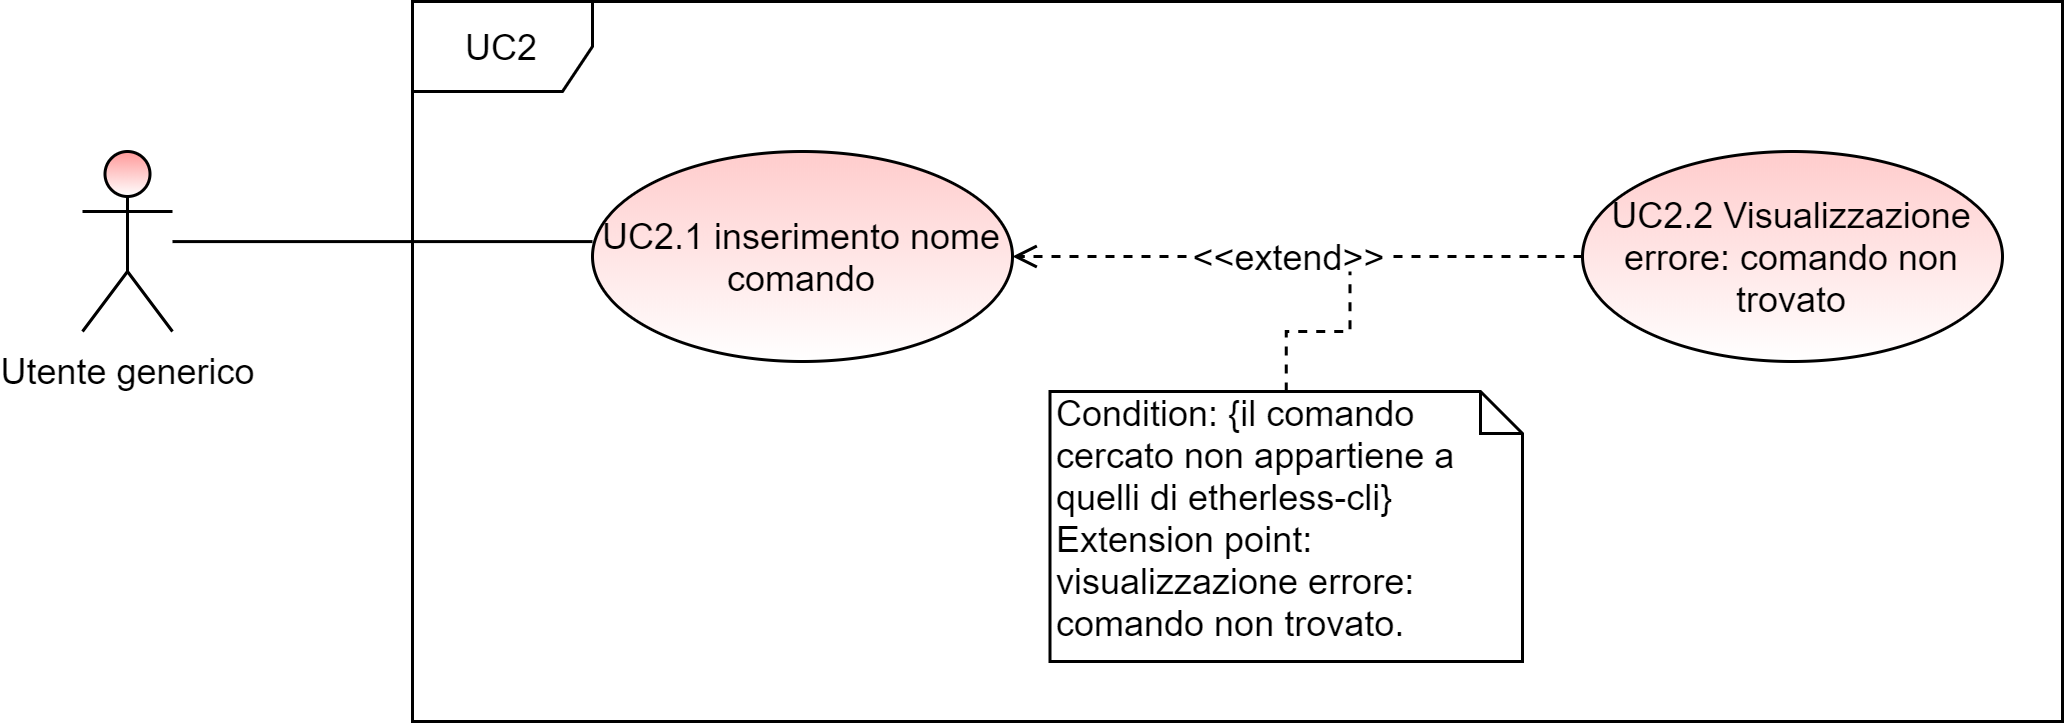
\includegraphics[scale=\ucs]{./res/img/UC2.png}
		\caption {UC2 - Aiuto comandi}
	\end{figure}
	\begin{itemize}
		\item \textbf{Attori primari:} \ug{};
		\item \textbf{Descrizione:} dopo aver inserito il comando \help{}, l’utente visualizza le informazioni dettagliate riguardo al comando desiderato;  
		\item \textbf{Scenario principale:} 
		\begin{itemize}
			\item l’utente inserisce il comando \phelp{};
			\item vengono visualizzate le informazioni dettagliate del comando richiesto. 
		\end{itemize}
		\item \textbf{Precondizione:} l’utente vuole ottenere maggiori informazioni riguardo ad un comando;
		\item \textbf{Postcondizione:} vengono visualizzate le informazioni dettagliate del comando di interesse.  
	\end{itemize}